\documentclass[letterpaper,12pt]{report}

\usepackage{graphicx}
\usepackage{hyperref}
\usepackage[top=1in, bottom=1in, left=1.25in, right=1in]{geometry}
\usepackage{float}

\setlength{\parindent}{0em}
\setlength{\parskip}{1em}

\hypersetup{
    colorlinks, %set true if you want colored links
    linkcolor=black,  %choose some color if you want links to stand out
}

\begin{document}
	\title{SYSC3010 T3 Project Proposal}
	\author{RC Camera Car}
	\date{}
	\maketitle

	\begin{abstract}
		The students developing this project are Alec D'Alessandro, Thao-Tran
		Le-Phuong, Honor Lopes, and Igor Veselinovic and the student numbers are
		101033378, 100997443, 101008909, 101011081. This document will outline
		the motivations, goals, and the proposed solution for the project, as
		well as the motivations for pursuing this project. The proposal will
		also provide the projected plan and milestones for the project.
	\end{abstract}

	\tableofcontents

	\pagebreak

	\section*{Motivation}
	\markright{}
	\addcontentsline{toc}{section}{Motivation}
	The purpose of this project is to create a remote-controlled vehicle in 
	order to explore locations that cannot be seen by the user. There are many
	locations inaccessible or unsafe for manned vehicles such as warzones, cave
	systems, and biohazard spaces. These are locations where it would be unsafe
	to send human drives and it would be preferable to send a remotely operated
	vehicle. This project would allow users to explore regions and places that
	are outside of their view.

	We would like to develop a basic version of the RC Camera Car for this
	project. The basic version should be a simple remote controlled car that
	connects over Wi-Fi and is easily controlled by a smart-phone app. This
	implementation could be expanded to work over a wireless communication
	technology so that the vehicle is less limited in range. Extended
	implementations would also include auxiliary equipment for performing 
	specific tasks or covering a wider range of terrain. The basic version of 
	this project would be suitable for recreational use. The extended version of
	this project could be applied in many fields such as science and military 
	applications.


	\section*{Problem Statement}
	\markright{}
	\addcontentsline{toc}{section}{Problem Statement}
	The overall goal for this project is for the car to be controlled via
	smart-phone through our designed android application. Once the user has
	registered with the car through the application there will be a live feed
	video source that is being transmitted from the car. The car could then be
	outfitted with additional auxiliaries needed for specific jobs. The car will
	also have automatic headlights to provide light in dimly lit areas.

	One limitation to the project development is how much bandwidth can be used
	for the live video feed stream from the car to the android application. A
	proposed solution to this would be to decrease video resolution for
	bandwidth reducing purposes, which would lead to mal visibility. A
	self-imposed constraint is on the complexity of the development of the car.
	This project will be focused on the vehicle controls and video feed. The car
	will be limited to Wi-Fi-enabled areas with even ground for this project.

	\section*{Proposed Solution}
	\markright{}
	\addcontentsline{toc}{section}{Proposed Solution}

	\begin{figure}[H]
    	\centering
		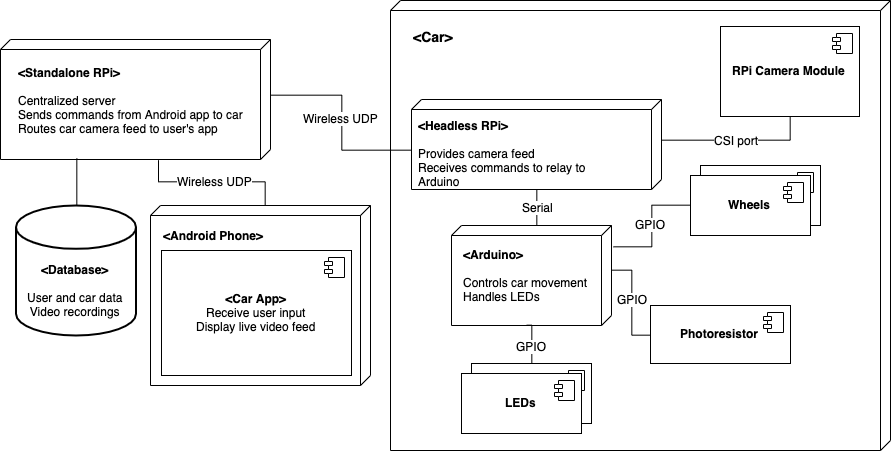
\includegraphics[width=\linewidth]{Proposal_UML_Diagram.png}
    	\caption{UML diagram for RC Camera Car system}
    	\label{fig:uml}
	\end{figure}

	The system design is shown in Figure \ref{fig:uml}. The UML diagram outlines
	the components necessary for implementation and the relationships between
	them. 

	Users will use the Android app to register their car to themselves and
	connect it to a Wi-Fi network. After the car is connected to Wi-Fi, users
	can control the car’s movements via the app as well as stream a video feed
	from and control the mounted camera. The video feed is to allow the user to
	control the car when it is not in sight. The app will also allow users to
	control the headlights of the car in case of dimly lit settings.

	There will be a Raspberry Pi that is connected to the Internet via Ethernet
	and acts as the centralized server. The server will have a database that
	will store the users, cars, and the pairings of users to cars. It will
	handle all of the commands coming from users and route them to their
	associated cars. Video feed from each car will be sent to the server to be
	sent to the proper user and can optionally be stored on a hard drive at the
	user’s request.

	The body of the car will contain an Arduino and a Raspberry Pi. The Arduino
	will control the movement of the car (steering, acceleration) and handle the
	headlights of the car (photoresistor sensor and LEDs). The photoresistor
	sensor will be polled regularly to monitor the light intensity of an area
	and the Arduino will automatically turn the headlights (LEDs) on or off
	based on threshold. The car movement will require motors to be connected to
	the Arduino and possibly a custom 3D printed chassis to hold all of the
	components. The car will use continuous tracks for propulsion as they will
	allow the car to traverse more types of terrain. The Raspberry Pi will be
	connected to a Wi-Fi network to receive user commands and relay them to the
	Arduino via a wired connection. The Raspberry Pi will also be connected to
	the camera and will stream the video feed to the centralized server.\\

	\begin{figure}[H]
    	\centering
		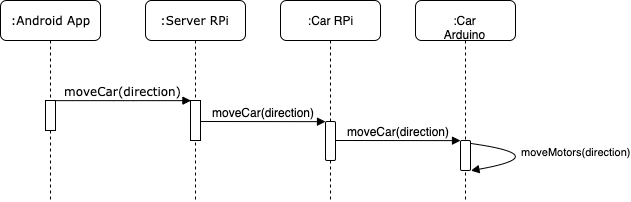
\includegraphics[width=\linewidth]{Proposal_Car_Movement_Sequence.png}
    	\caption{Sequence diagram of the user moving the car}
    	\label{fig:movement}
	\end{figure}

	Figure \ref{fig:movement} describes the process that takes place when
	the user controls the movement of the car. The user will indicate the
	direction and speed that the car should go through the Android application.
	The app will then send the direction and speed wirelessly to the server
	which will route the commands to the RC car registered to the user. The
	Rasberry Pi on the car will receive the commands and relay them to the
	Arduino via a direct serial connection. The Arduino will adjust the speeds
	of the motors to reach the specified speed and direction.

	\begin{figure}[H]
    	\centering
		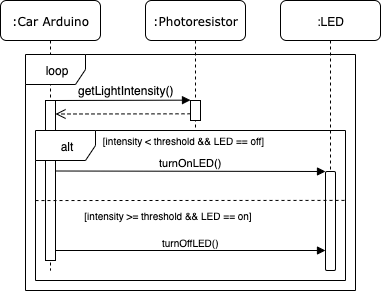
\includegraphics[width=0.75\linewidth]{Proposal_Automatic_Headlights_Sequence.png}
    	\caption{Sequence diagram of the automatic headlights}
    	\label{fig:headlights}
	\end{figure}

	The process of the automatic headlights is shown in Figure
	\ref{fig:headlights}. The Arduino will regularly read the analog output of
	the photoresistor to determine the intensity of the light in the car's
	environment. Based on the intensity compared to a certain threshold, the
	Arduino will turn the headlights on or off.

	\begin{figure}[H]
    	\centering
		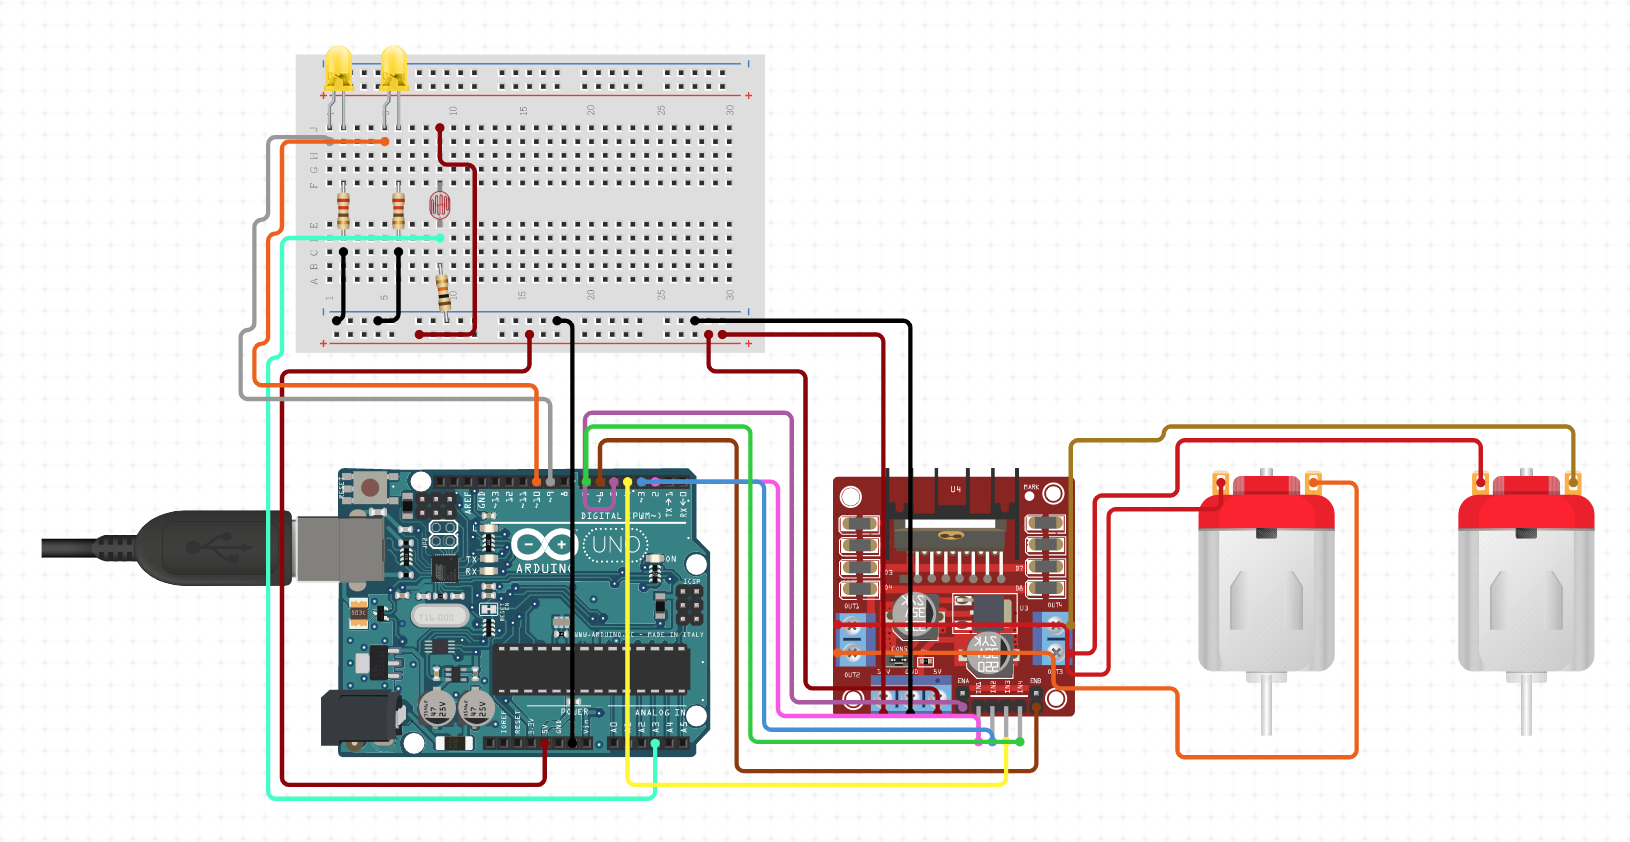
\includegraphics[width=\linewidth]{Proposal_Wiring_Diagram.png}
    	\caption{Wiring diagram for Arduino of RC Camera Car system}
    	\label{fig:wiring}
	\end{figure}

	The wiring diagram for the system is shown in Figure \ref{fig:wiring}. In
	the diagram, the Arduino is connected to two LEDs that will act as the
	headlights, a photoresistor to sense the brightness of the area, and an
	H-bridge motor driver and two motors to control the driving.

	\section*{Project Plan}
	\markright{}
	\addcontentsline{toc}{section}{Project Plan}
	Our remote-controlled car system has three main components that can be
	developed mostly in parallel. The car itself and the basic I/O components
	that provide the core functionality (i.e, the motors, light sensors, and
	headlights) make up one grouping of work. All handling of video, including
	interfacing with the camera, streaming, and long-term storage, is another
	main thread of work. The last central component to this system is the
	Android application which must have a GUI and needs to be tested differently
	since it is user-facing. Testing is a vital component of each stream of work
	and will be done throughout the development process of all software.

	There are obvious interdependencies between section of work such as the
	Android application needing to receive video from the Raspberry Pi server
	and the Android application sending movement commands to the car. Even after
	testing components independently, new bugs and issues might arise once
	separate components are integrated together. Thus, beyond the unit testing
	of individual components, integration testing will need to be done at every
	stage of the system’s development.

	Each member of the group will be working on all aspects of the project.
	There will also be a shared leadership role and for every meeting, there
	will be a recordkeeper that wil be rotated between each member.

	\subsection*{Milestones}
	\markright{}
	\addcontentsline{toc}{subsection}{Milestones}
	The development and testing milestones are shown below.\par

	\underline{Legend}:

	\setlength{\parskip}{0em}
	\setlength{\baselineskip}{1em}

	\begin{itemize}
		\item[] \textbf{CAR}: Remote-controlled car
		\item[] \textbf{VID}: Video streaming and storage
		\item[] \textbf{AND}: Android application
		\item[] \textbf{TST}: Testing
	\end{itemize}\vspace{1em}

	\noindent\rule[0.5em]{\textwidth}{0.5pt}
	\textbf{Oct. 7 - Oct. 20}\\
	\noindent\rule{\textwidth}{0.5pt}
	\begin{itemize}
		\item Explore and research possible implementations
		\item Design car, server, and Android application systems
	\end{itemize}
	\noindent\rule[0.5em]{\textwidth}{0.5pt}
	\textbf{Oct. 21 - Oct. 27}\\
	\noindent\rule{\textwidth}{0.5pt}
	\begin{itemize}
		\item \textbf{[CAR]} Acquire/build all components for the system
			(camera, tracks/wheels, chassis, motor, etc.)
		\item \textbf{[CAR]} Develop a codebase for controlling the car’s
			wheels/tracks using motors to allow for forward/backward movement
			and turning
		\item \textbf{[CAR, TST]} Develop a comprehensive unit test suite of the
			car movement control code
		\item \textbf{[CAR, TST]} Manually test and fine-tune the car movement
			control code
	\end{itemize}
	\noindent\rule[0.5em]{\textwidth}{0.5pt}
	\textbf{Oct. 28 - Nov. 3}\\
	\noindent\rule{\textwidth}{0.5pt}
	\begin{itemize}
		\item \textbf{[CAR]} Set up periodic checks of environment light levels
			using the light sensor and adjust the brightness of the headlights
			accordingly
		\item \textbf{[CAR, TST]} Develop a comprehensive unit test suite of the
			light control code
	\end{itemize}
	\noindent\rule[0.5em]{\textwidth}{0.5pt}
	\textbf{Nov. 4 - Nov. 10}\\
	\noindent\rule{\textwidth}{0.5pt}
	\begin{itemize}
		\item \textbf{[CAR]} Send movement commands from centralized Raspberry
			Pi server to the car’s Raspberry Pi, relay them to the Arduino, and
			power the corresponding motor(s)
		\item \textbf{[CAR, TST]} Develop a comprehensive unit test suite of the
			networking code
	\end{itemize}
	\noindent\rule[0.5em]{\textwidth}{0.5pt}
	\textbf{Nov. 11 - Nov. 17}\\
	\noindent\rule{\textwidth}{0.5pt}
	\begin{itemize}
		\item \textbf{[VID]} Send video data from the car’s Raspberry Pi to the
			centralized Raspberry Pi and relay the stream to clients
		\item \textbf{[VID]} Store video clips on an external hard drive and
			track the files using an SQL database
		\item \textbf{[VID, TST]} Develop a comprehensive functional test suite
			of the video streaming and storage code
	\end{itemize}
	\noindent\rule[0.5em]{\textwidth}{0.5pt}
	\textbf{Nov. 18 - Nov. 24}\\
	\noindent\rule{\textwidth}{0.5pt}
	\begin{itemize}
		\item \textbf{[AND, CAR]} Send commands to the centralized Raspberry Pi
			server based on inputs to the Android application GUI that will then
			be relayed to the car
		\item \textbf{[AND, VID]} Receive and play video streams and recorded
			clips from the centralized Raspberry Pi server in the Android
			application GUI
		\item \textbf{[AND, TST]} Develop a sanity test suite of the GUI of the
			Android application
		\item \textbf{[AND, TST]} Develop a comprehensive unit test suite of the
			Android application code
	\end{itemize}
	\noindent\rule[0.5em]{\textwidth}{0.5pt}
	\textbf{Nov. 25 - Dec. 6}\\
	\noindent\rule{\textwidth}{0.5pt}
	\begin{itemize}
		\item \textbf{[TST]} Verification and integration testing for entire
			system
		\item \textbf{[AND, VID, CAR]} Complete issue backlog
	\end{itemize}
\end{document}
